% !TEX TS-program = xelatex
% !BIB program = bibtex
% !TEX encoding = UTF-8 Unicode

\documentclass[
  twoside,
  openright,
  degree    = master,               % degree = master | doctor
  language  = english,              % language = chinese | english
  fontset   = template,             % fontset = default | template | system | overleaf
  watermark = true,                 % watermark = true | false
  doi       = true,                 % doi = true | false
]{ntuthesis}

\usepackage{minted}
\setminted{
    linenos,
    breaklines,
    framesep=0pt,
    fontsize=\scriptsize,
    numbersep=5pt,
    xleftmargin=5pt,
}

\usepackage{listings}
\newcommand{\rustsec}{KrustVM}
\newcommand{\rustcore}{Rcore}
\newcommand{\secore}{Kcore}
\definecolor{CodeGray}{RGB}{60, 60, 60}
\newcommand{\code}[1]{\texttt{\textcolor{CodeGray}{#1}}}
\newcommand{\todo}[1]{\textcolor{red}{#1}}

% !TeX root = ./main.tex

% --------------------------------------------------
% 資訊設定(Information Configs)
% --------------------------------------------------

\ntusetup{
  university*   = {National Taiwan University},
  university    = {國立臺灣大學},
  college       = {電機資訊學院},
  college*      = {College of Electrical Engineering and Computer Science},
  institute     = {資訊工程學系},
  institute*    = {Department of Computer Science and Information Engineering},
  title         = {實作基於Rust之安全Linux KVM虛擬機器監測器},
  title*        = {On Implementing a Secure Rust-based Linux KVM Hypervisor},
  author        = {章瑋麟},
  author*       = {Wei-Lin Chang},
  ID            = {R09922117},
  advisor       = {黎士瑋},
  advisor*      = {Shih-Wei Li},
  date          = {2023-07-11},         % 若註解掉,則預設為當天
  oral-date     = {2023-07-11},         % 若註解掉,則預設為當天
  DOI           = {10.6342/NTU202301822},
  keywords      = {系統安全, 虛擬化, KVM},
  keywords*     = {System Security, , Virtualization, KVM},
}

% --------------------------------------------------
% 加載套件(Include Packages)
% --------------------------------------------------

\usepackage[sort&compress]{natbib}      % 參考文獻
\usepackage{amsmath, amsthm, amssymb}   % 數學環境
\usepackage{ulem, CJKulem}              % 下劃線、雙下劃線與波浪紋效果
\usepackage{booktabs}                   % 改善表格設置
\usepackage{multirow}                   % 合併儲存格
\usepackage{diagbox}                    % 插入表格反斜線
\usepackage{array}                      % 調整表格高度
\usepackage{longtable}                  % 支援跨頁長表格
\usepackage{paralist}                   % 列表環境


\usepackage{lipsum}                     % 英文亂字
\usepackage{zhlipsum}                   % 中文亂字

% --------------------------------------------------
% 套件設定(Packages Settings)
% --------------------------------------------------


\begin{document}

% 封面與口試審定
% Cover and Verification Letter
\makecover                          % 論文封面(Cover)
\makeverification                   % 口試委員審定書(Verification Letter)

% 致謝與論文摘要
% Acknowledgement and Abstract
% !TeX root = ../main.tex

\begin{acknowledgement}

%首先,我要感謝我的指導教授黎士瑋博士,您帶領我走過一遍碩士班的研究過程,讓我受益良多。
%您在研究期間的建議不僅帶給我研究上的進展,其蘊含的分析角度也常比我自己的想法還更全面且有條理,讓我評斷一件事情的時候有更完整的思考。
%在撰寫論文的這幾個月,您不厭其煩的替我審閱我的論文,指出我文字描述中的邏輯謬誤和解釋不清之處,使得我的學術寫作及邏輯闡述能力更加精進。
%
%本論文的完成亦得感謝擔任我口試委員的黃敬群 (jserv) 教授與蕭旭君教授,因為你們的建議與意見,使得我的論文能夠更完整且嚴謹。
%
%另外感謝江昱勳與杜展廷同學,沒有你們的貢獻與合作,KrustVM的研究與投稿論文不會順利地完成。
%
%我也要感謝我的家人和朋友們,有你們的支持我才能完成論文。
%
%此外,特別感謝 OpenAI 的 ChatGPT,它不厭其煩的幫助我優化了論文的英文表達,許多論文中的字句 (包含了本致謝) 得益於它才能夠如此通順,清晰和流暢。
%
%最後,謹以此文獻給逝去的歲月。

首先,我要衷心感謝我的指導教授黎士瑋博士。在研究期間,您的指導和建議讓我受益匪淺。
您在研究期間的建議不僅帶給我研究上的進展,其蘊含的分析角度也常比我自己的想法還更全面且有條理,讓我學到評斷一件事情更完整的思考方式。
在撰寫論文的過程中,您不辭辛勞地審閱我的稿件,指出其中的邏輯謬誤和解釋不清之處,使我在學術寫作和邏輯闡述方面精進了許多。

本論文的完成亦得感謝擔任我口試委員的黃敬群 (jserv) 教授與蕭旭君教授,您們的寶貴意見和建議使得我的論文更加完整和嚴謹。
此外,感謝江昱勳與杜展廷同學的合作和貢獻,沒有你們的協助, KrustVM 的研究和論文投稿將不會如此順利地完成。
我也要衷心感謝我的家人和朋友們,是你們的支持讓我能夠順利完成論文。

特別感謝 OpenAI 的 ChatGPT,它不厭其煩地幫助我優化論文的英文表達。
許多論文中的文字,包括本致謝部分,都得益於它,使得我的論文變得更加通順、清晰和流暢。

最後,謹以此文獻給逝去的歲月。
\begin{flushright}
章瑋麟\\
%國立臺灣大學資訊工程學系暨研究所\\
中華民國一百一十二年七月
\end{flushright}

\end{acknowledgement}
       % 致謝(Acknowledgement)
% !TeX root = ../main.tex

\begin{abstract}

中文摘要

\end{abstract}

\begin{abstract*}

Commodity hypervisors play a vital role in cloud computing environments by
overseeing hardware resources for virtual machines. However, their growing
complexity and extensive attack surface pose significant security concerns.
An attacker that exploits vulnerabilities in the privileged hypervisor
codebase can gain unfettered access to VM data, compromising their safety.
Previous attempts to retrofit hypervisors into small trusted cores have
limitations, as the security still relies on the implementation of the trusted
core. Moreover, formal verification on the TCB necessitates significant human
effort and is not easily applicable to rapidly evolving codebases.
Recently, Rust adoption has been increasing for its strong memory safety
guarantees and performance efficiency.
This thesis addresses challenges in rewriting and porting the C-based KVM TCB
in SeKVM to Rust for a recent Linux long term support version. This allows the
resulting hypervisor, \rustsec{}, to not only benefit from recent Linux
advancements, but also be protected by Rust's safety guarantees.
Furthermore, the Rust-based implementation can be conveniently updated,
as Rust conducts safety checks at compile-time automatically.
%This thesis explores leveraging Rust to build a secure commodity hypervisor.
%We focus on rewriting SeKVM into KrustVM.
In \rustsec{}, a small trusted core written in Rust is incorporated to replace
the C-based core of SeKVM, which serves to protect VM confidentiality and
integrity.
%During the implementation of \rustsec{},
%we addressed challenges in linking a Rust TCB into Linux, rewriting SeKVM's
%C-based TCB in Rust, and bringing up \rustsec{} on real hardware.
%\rustsec{} incorporates
%\rustcore{}, a small trusted core written in Rust to protect VM confidentiality
%and integrity.
In addition,
a modular design is adopted to secure the trusted Rust core. We separated and
minimized the unsafe Rust code from safe Rust by enclosing unsafe code within
safe abstractions, and utilized Rust's type system to ensure the memory safety
of the unsafe memory accesses done by the trusted Rust core.
%[Then you focus on briefly disuss what you actually do -- enclosed unsafe code etc.]
%In addition,
%we minimized unsafe Rust usage, enclosed unsafe code within safe abstractions,
%and utilized Rust's type system to ensure the memory safety of unsafe
%operations in \rustcore{}.
\rustsec{} incurs modest overhead compared to mainline KVM and SeKVM, and
demonstrates the practicality of securing existing hypervisors through a
C-to-Rust rewrite.

\end{abstract*}
              % 摘要(Abstract)

% 生成目錄與符號列表
% Contents of Tables and Denotation
\maketableofcontents                % 目錄(Table of Contents)
\makelistoffigures                  % 圖目錄(List of Figures)
\makelistoftables                   % 表目錄(List of Tables)
% !TeX root = ../main.tex

\begin{denotation}[3cm]

\item[HPC]{
  高性能計算 (High Performance Computing)
}

\item[cluster]{
  集群
}

\item[Itanium]{
  安騰
}

\item[SMP]{
  對稱多處理
}

\item[API]{
  應用程序編程接口
}

\end{denotation}
            % 符號列表(Denotation)

% 論文內容
% Contents of Thesis
\mainmatter
% !TeX root = ../main.tex

\chapter{Introduction}

Hypervisors are essential to cloud computing. They manage the hardware
resources to provide the virtual machine (VMs) abstraction and host
these VMs in the cloud.
The widely used commodity
hypervisors, such as KVM~\cite{kivity07kvm} or Hyper-V~\cite{hyperv},
include a large and complex TCB to satisfy users' requirements in
performance and functionality. These hypervisors were written in unsafe
languages like C, making them vulnerable to safety bugs, such as
out-of-bound memory access and use-after-free. For example, KVM
integrates an entire Linux OS kernel inside its TCB. Attackers that
successfully exploit hypervisor vulnerabilities may gain the ability
to steal or modify secret VM data.

Previous work HypSec~\cite{hypsec} has retrofitted commodity hypervisors into a
small trusted core that enforces resource access control to ensure the
confidentiality and integrity of VM data against hypervisor and host operating
system exploits. However, the security of the whole system still depends on the
implementation of the small trusted TCB. Any vulnerability in the trusted TCB
can void the guarantees of VM data confidentiality and integrity.
While SeKVM~\cite{sekvm} extended the work of HypSec~\cite{hypsec} by formally
verifying the smaller TCB, the scalability of the approach is limited as formal
proofs only validate specific implementations, and as the codebase evolves to
incorporate new features or undergo code refactoring, the existing proof
becomes outdated, necessitating a new proof for any code modifications.

Rust is an emerging programming language that ensures strong memory safety
guarantees at compile time while offering performance efficiency.
Its distinctive ownership and lifetime system
effectively addresses potential safety issues that programmers may encounter.
Rust prevents various memory safety bugs, for example, null pointer
dereferences are eliminated by distinguishing between nullable and non
nullable types, nullable types are not allowed by default, array out-of-bound
accesses are prevented by runtime checks that are added by the compiler, and
Rust's ownership system prevents dangling pointers.
Further, similar to programming languages like C, Rust allows developers to
directly manage low-level systems resources such as memory. Due to these
attributes, various previous work has adopted Rust to implement systems
software with critical security and performance requirements, including
operating systems~\cite{NrOS, Redleaf, TockOS, theseus},
hypervisors~\cite{DuVisor, RustyHermit}, web browsers~\cite{servo},
and TEEs~\cite{rustsgx,rustee}.
There has been recent adoption of Rust in the mainline Linux kernel. However,
instead of replacing the existing Linux kernel code written in C with Rust,
the current efforts were limited to developing new Rust-based device drivers.

%Our work explores implementing a Linux KVM TCB in Rust, so that the resulting hypervisor
%benefits from the strong safety guarantees that Rust provides.
%Our work leverages the Rust programming language and rewrite SeKVM \cite{sekvm},
%a secure Linux KVM hypervisor in Rust, so that the resulting hypervisor
%benefits from the strong safety guarantees that Rust automatically provides.
We have developed \rustsec{} for Linux 5.15, a Rust-based secure Linux KVM hypervisor.
\rustsec{} reimplemented SeKVM \cite{sekvm} and replaced SeKVM's verified TCB
with a Rust-based TCB, called \rustcore{}.
% KRUSTVM DESCRIPTION
\rustsec{} incorporates the small Rust TCB \rustcore{} to
protect VM confidentiality and integrity against the large and untrusted
hypervisor codebase that encompasses KVM’s host Linux kernel.
% KRUSTVM DESCRIPTION END
% RUST BASED ADVANTAGES
\rustsec{} benefits from the strong safety guarantees that Rust provides.
Its Rust-based TCB also eliminates the need for repeated verification each time the
code is changed, since the compiler automatically guarantees memory safety each
time the code is compiled, allowing for a flexible codebase while maintaining
a secure implementation.
We ported the Linux 4.18-based SeKVM to Linux 5.15, a recent version of
long-term-support Linux, for \rustsec{}. This allows us to take advantage of
new kernel features, including Link-Time-Optimization (LTO) and energy-aware
scheduling.
% RUST BASED ADVANTAGES END
% CHALLENGES
During the development of \rustsec{}, we identified and overcame challenges
that arose when trying to rewrite and port SeKVM's TCB to Rust for Linux 5.15.
Firstly, the Linux kernel had undergone many changes between version 4.18 and
5.15, such as feature addition and kernel API changes. Therefore, we need to
forward port SeKVM to Linux 5.15 prior to initiating the Rust rewrite process.
Second, Linux 5.15 does not support Rust as a development language, meaning
Rust code can not be linked with the rest of the kernel by the Linux build
system. To resolve this challenge, we rolled our own Makefile and integrated
the build process of our Rust code with Linux's build system.
Third, writing a KVM TCB in a new language like Rust poses many language
compatibility issues. For example, C headers are not usable in Rust, and name
mangling exists in Rust but not in C, etc. We must address each issue  for our
implementation to work.
% CHALLENGES END
%incorporate a Rust TCB inside Linux, rewrite SeKVM's TCB in Rust, and bring up
%\rustsec{} on real hardware.
%We build upon the work of SeKVM \cite{sekvm} and forward ported SeKVM
%from Linux 4.18 to Linux 5.15, to take advantage of new kernel features
%including Link-Time-Optimization (LTO) and energy-aware scheduling.
%SeKVM's
%verified TCB \textit{\secore{}} is then rewritten in Rust, which is called
%\textit{\rustcore{}}.
%The resulting hypervisor, \rustsec{}, incorporates the small Rust TCB
%\rustcore{} to
%protect VM confidentiality and integrity against the large and untrusted
%hypervisor codebase that encompasses KVM’s host Linux kernel.
Aside from the Rust-based KVM TCB implementation challenges, we also
implemented \rustcore{} in a way such that the amount of unsafe Rust is
minimized.
Unsafe code are enclosed within a safe abstraction and a safe API is exposed
in order to implement complex functionalities in safe Rust, including CPU,
memory, VM boot protection, VM exit, and hypercall handlers.
Further, raw pointer accesses, which are unsafe in Rust, are protected using
Rust’s type system. In \rustcore{}, raw pointers are used for accessing
physical memory. Physical memory is divided into multiple disjoint regions,
and the \rustcore{} implementation guarantees that all memory accesses done by
\rustcore{} are located in the predefined regions, ensuring that bugs caused by
pointers pointing to incorrect memory regions are prevented.
This involves transforming raw pointers into references, allowing Rust to
automatically insert runtime checks for out-of-bound array indices, and
building customized Rust types that enforce bound-checking for raw pointer
accesses.
%This is done in two parts, for raw pointer accesses to the region which stores
%metadata used by \rustcore{}, called the \textit{\rustcore{} metadata region},
%these accesses are bound via a set of reference getter functions (RGF).
%Each RGF wraps a given Rcore’s raw pointer usage and returns a mutable
%reference to the associated shared metadata object after the caller acquires
%the corresponding lock. Because the raw pointer is turned into a mutable
%reference, the memory accessed is guaranteed to be bound by the size of the
%type being referenced, for arrays, the compiler automatically adds runtime
%checks that checks for out-of-bound array indices.
%For raw pointer accesses to the other regions, we built customized Rust types
%for each memory region that enforces bound-checking, and \rustcore{} accesses
%each memory region via the corresponding type.

%This is achieved with customized Rust types for each memory region that
%enforces bound-check to accesses, and mandating that \rustcore{} accesses a
%memory region via each corresponding type.

% describe the benefits
%We spent less than one person year rewriting SeKVM into \rustsec{}.
By rewriting a C-based hypervisor to a Rust-based implementation,
the responsibility of human auditing is shifted to the compiler.
By enforcing Rust's safety rules, the compiler ensures that memory bugs are
prevented, alleviating the need for developers to manually audit for such
issues or perform formal verification.
This results in safer code and a more straightforward development process.
Performance evaluation of \rustsec{} on real Arm64 hardware shows that
\rustsec{} incurs modest performance overhead to application workloads
compared to mainline KVM and SeKVM. We demonstrate the practicality of
securing an existing commodity hypervisor by a C-to-Rust rewrite.

The rest of the thesis will be organized as follows. Background
will be reviewed in \autoref{sec:bg}. Our threat model and assumptions are
listed in \autoref{sec:threatmodel}. The process of implementing a Rust TCB
for KVM and the techniques used are described in \autoref{sec:rewrite}.
\autoref{sec:securercore} presents how Rust's safety features are utilized to
design and secure \rustcore{} memory accesses.
Evaluation of \rustsec{} and its comparison with mainline KVM and SeKVM is
covered in \autoref{sec:eval}. Related work and future work are discussed in
\autoref{sec:rwfw}. Discussion of this work is presented in \autoref{sec:discussion}.
At last, we conclude the thesis in \autoref{sec:conclusions}.

% !TeX root = ../main.tex
%\raggedbottom

\chapter{Background}
\label{sec:bgrw}

\section{SeKVM}
%\todo{TODO: WIP, and introduce \rustsec{} design here.}
%Various previous work~\cite{lisosp21,zhang2011cloudvisor,zeyu20usenix,pkvm,fidelius-hpca18,sekvm}
%redesigned the hypervisor to protect VMs.
Our work explores the possibility of rewriting a hypervisor TCB in Rust, we
chose to base on the implementation of SeKVM \cite{sekvm}, because its artifact
\cite{sekvm-artifact} is available, and also because it has a reduced TCB
compared to mainline KVM, which minimizes the attack surface of the codebase,
leading to a more secure hypervisor.
SeKVM is a formally verified KVM hypervisor,
it leveraged an earlier design~\cite{hypsec} to retrofit and secure KVM,
it relies on a small TCB called \secore{} to protect VM confidentiality and
integrity against an untrusted KVM host that encompasses the host Linux kernel
integrated with KVM.
To reduce the TCB,
the design separates access control from resource allocation. \secore{}
has full access to hardware resources to perform access control to
protect VM data. SeKVM assumes VMs employ an end-to-end approach to
encrypt I/O data. Since VMs already protect their I/O data, SeKVM
focuses on protecting VM data in CPU and memory.
The KVM host provides device drivers and complex virtualization features
such as resource allocation, scheduling, and VM management. \secore{} is
responsible for protecting VM data, ensuring VM CPU registers and memory
allocated to the VM are inaccessible to the untrusted KVM host.

\secore{} leverages hardware virtualization
support to deprivilege the KVM host at a lower privileged level, ensuring
the untrusted host cannot disable or control privileged hardware
features. \secore{} enables the nested page tables (NPT) when running
the KVM host and VMs so that they do not have direct access to physical
memory.
\secore{} unmaps its own private memory pages from the respective NPTs,
making them inaccessible
to VMs and the host. \secore{} unmaps a given VM's memory pages from
the KVM host's or other VMs' NPTs to isolate these pages.
\secore{} allocates NPTs for the KVM host
and VMs from its memory pool, to which the host and VMs have no access.
Since VM and \secore{} memory is unmapped from the host NPT, a
compromised host that accesses these memory pages causes an NPT fault
that traps to \secore{}. \secore{} routes NPT faults to itself,
allowing it to reject invalid host memory accesses.

SeKVM reuses the device drivers from the KVM host to manage
I/O devices and provide I/O virtualization. An attacker from the host
can control devices to perform Direct Memory Access (DMA) to
read or write VM memory. To protect VM memory against such DMA
attacks, SeKVM leverages IOMMU to restrict all devices'
memory accesses. \secore{} allocates and manages IOMMU page
tables from its private memory. \secore{} trap-and-emulates the
KVM host's access to the IOMMU and manages the IOMMU page tables
for each DMA-capable device.

\secore{} runs in a higher privileged CPU mode than the host to
interpose VM exits and interrupts, ensuring the host cannot compromise
VM data.
VM exit handling may require the KVM host's functionality. Before
entering the host, \secore{} saves VM CPU registers from the
hardware to its private memory then restores the host's CPU registers to
the hardware; vice versa is done before entering the VM. An attacker has
no access \secore{}'s private memory, and thus, the VM CPU registers.

SeKVM leverages Arm's hardware Virtualization Extensions (VE) to
simplify its implementation. \secore{} runs in the hypervisor mode
(EL2) to control Arm VE features to deprivilege the KVM host in a less
privileged kernel mode (EL1). \secore{} uses Arm's NPTs, stage 2
page tables to enforce memory access control. Stage 2 page table
translation only affects the software running in Arm's kernel and user
(EL0) mode, but not software running in EL2. \secore{} employs an
identity map in the KVM host's stage 2 page tables, translating each
host machine's physical addresses (hPA) to an identical hPA. This
allows SeKVM to reuse Linux's memory allocator to manage memory
implicitly. Running in EL2 allows \secore{} to isolate itself
from the host and VMs. First, running in EL2 isolates \secore{} in
a separate address space from EL1 and EL0. Second, Arm provides banked
system registers to EL1 and EL2. The host cannot access
EL2 registers to disable \secore{}'s protection. For instance,
the host cannot modify the register VTTBR\_EL2, which stores the base
address of the stage 2 page tables. \secore{} exposes a set of
required hypercalls~\cite{hypsec} for the host to request services
that require EL2 privileges. For example, once the host schedules
a virtual CPU, it makes a hypercall to \secore{} to context switch to
the VM. \secore{} leverages Arm's IOMMU, the System Memory
Management Unit (SMMU)~\cite{smmu-whitepaper}, to protect against
DMA attacks.

%Unlike our work, none of them used
%Rust to secure their hypervisor implementation.
%\rustsec{} and SeKVM~\cite{sekvm} both leveraged an earlier design~\cite{hypsec}
%to retrofit and secure KVM, providing the same level of VM protection. SeKVM
%included a formally verified core to protect VMs against an untrusted host Linux
%kernel, while \rustsec{} relies on a Rust-based \rustcore{} to protect VMs.
%Formal verification of the concurrent C-based SeKVM core requires significant effort.
%The authors took two person-years to complete the correctness and security proofs.
%In contrast, our Rust-based implementation took less than one person-year while
%ensuring properties verified systems provide, including memory safety,
%data race, and deadlock freedom.

\section{The Rust Programming Language}
Rust, compared to C,
is a relatively young programming language aiming to be safe and fast.
It enables programs to be memory-safe without requiring programmers to
painstakingly manage memory, as in traditional languages (e.g., C/C++).
Unlike other memory-safe languages (e.g., Python, Go, etc.),
Rust does not leverage garbage collection mechanisms
to ensure memory safety.
Instead, it introduces the concepts of lifetimes and ownership
to mandate the programmer to follow specific rules.
This paradigm of statically enforcing programming rules
empowers Rust to perform comparably to C since Rust's compiler has complete
control over the code that
runs during runtime and can optimize it accordingly.
Additionally, Rust's safety rules ensure that
no memory safety bugs will be present when satisfied,
and the compiler automatically checks and prevents any violation of these rules.

\textbf{Ownership and Lifetimes.}
In Rust, each piece of data is said to be \textit{owned} by a single
variable, and it is automatically \textit{dropped} (freed) when the
variable's \textit{lifetime} ends. A variable's lifetime ends as the program
control flow exits the block in which the variable is declared.
In \autoref{lst:lifetime}, \code{y}'s lifetime starts at line 5 and ends at
line 7 as the block closes. Hence, the \code{println!} macro is unable to find
the value \code{y}, whose lifetime has already ended.
Ownership can be transferred or \textit{moved}. For example,
assigning the owning variable to a new variable moves the ownership of the
data to the new variable. And passing the variable into a function also moves
the data ownership into the function.
In both situations, the original variable returns to the uninitialized state,
and using it would result in a compilation error.

\begin{listing}[hbtp]
    \begin{minted}{rust}
// this code sample does *not* compile
{
  let x = 1;
  {            // create new scope
    let y;
    y = x;
  }            // y is dropped

  // compilation error, y's lifetime has ended
  println!("The value of 'y' is {}.", y);
}
    \end{minted}
    \caption{Rust lifetime example}
    \label{lst:lifetime}
    \vspace{-0.2cm}
\end{listing}

\textbf{Borrowing.}
Ownership lacks the flexibility of argument passing.
Rust addresses this by \textit{borrowing},
a mechanism that allows accessing data without gaining ownership.
A variable can borrow ownership from another variable to acquire a
\textit{reference} to the data. References can be divided into two categories,\textit{shared}
references and \textit{exclusive} references. The reference can only be read
and not modified with a shared reference. Nevertheless, multiple shared
references for a specific value can be held simultaneously.
On the other hand, exclusive references allow reading from and modifying the
value. However, having any other kind of reference active simultaneously for
that value is not permitted.

In summary, Rust's borrowing rule enforces \textit{aliasing xor mutability}
meaning there can be multiple shared references or a single exclusive
reference.
In \autoref{lst:borrowingrule}, line 6 would not compile because it tries to create
a mutable reference (\code{z}) to \code{x}, while \code{y} already borrowed
\code{x} immutably. \code{y}'s lifetime ends on line 8 as it gets used for the
last time; therefore \code{z} can be created on line 10 and used on line 11.
However, if line 13 is uncommented, \code{y}'s lifetime would be extended to
line 13, making the creation of \code{z} on line 10 break the borrowing rules.

\begin{listing}[hbtp]
    \begin{minted}{rust}
{
  let mut x = vec![1, 2, 3];
  let y = &x; // immutable borrow of x

  // this line would fail to compile because x is already borrowed immutably by y
  /* let z = &mut x; */

  println!("x = {:?}", x); // This line works
  println!("y = {:?}", y); // This line works

  let z = &mut x; // mutable borrow of x
  z.push(4);

  // this line would fail to compile because x is borrowed mutably by z
  /* println!("y = {:?}", y); */
}
    \end{minted}
    \caption{Rust enforces \textit{aliasing xor mutability}}
    \label{lst:borrowingrule}
    \vspace{-0.2cm}
\end{listing}

\textbf{unsafe Rust.}
Rust's safety checks are sometimes too restrictive regarding tasks like
low-level hardware access or special optimizations. These operations are
inherently unsafe and hence impossible to follow the rules mandated by Rust.
However, they are still necessary for low-level software such as
hypervisors. To provide flexibility for these operations, Rust allows
parts of the program to opt out of its safety checks via the \textit{unsafe}
keyword. Traits, functions, and code blocks can be marked as unsafe to disable
the checks that the compiler would normally enforce. However, using unsafe code
also means that the responsibility for ensuring memory safety is shifted from
the compiler to the programmer. Therefore, it is crucial to exercise
caution when using unsafe code to avoid introducing bugs or security
vulnerabilities.

\textbf{Interior unsafe.}
While most low-level code is written in unsafe code, Rust introduces
the concept of \textit{interior unsafe}~\cite{ruststudy}. A function is considered
interior unsafe if it exposes a safe interface but contains unsafe blocks
in implementation. This allows unsafe operations to be encapsulated
into safe abstractions. For instance, in
\autoref{lst:interiorunsafe}, Rust's \code{replace} function can be
called by safe Rust, but it is implemented using unsafe raw pointer operations.
At line 6, \code{ptr::read} is used to copy a bit-wise value from \code{dest}
into \code{result} without moving it, and at line 7, \code{ptr::write} overwrites
the memory location pointed to by \code{dest} with the given value \code{src}
without reading or dropping the old value. Lastly, at line 8, \code{result} is
returned to the function's caller.

\begin{listing}[hbtp]
    \begin{minted}{rust}
pub const fn replace<T>(dest: &mut T, src: T) -> T {
  // SAFETY: We read from `dest` but directly write `src` into it afterward,
  // such that the old value is not duplicated. Nothing is dropped and
  // nothing here can panic.
  unsafe {
    let result = ptr::read(dest);
    ptr::write(dest, src);
    result
  }
}
    \end{minted}
    \caption{interior unsafe in Rust's \code{replace} function}
    \label{lst:interiorunsafe}
    \vspace{-0.2cm}
\end{listing}

This leads to a design practice that interior unsafe functions should provide
the necessary checks that prevent the unsafe code from producing any undefined
behavior or memory safety bugs.
The callee in the safe world hence bears no responsibility to ensure safety.

\textbf{Interior Mutability.}
Mutating the underlying data via an immutable reference
is forbidden in Rust.
However, this might be too restrictive for
implementing efficient algorithms or data structures.
For example, programmers might want to add a cache
in a read-only search data structure
to optimize the search time.
Nevertheless, updating the state of the cache implies
the need for mutability,
which violates the read-only constraint.
Hence, we need the ability to mutate states even under a read-only scene.
To address this issue,
the Rust standard library provides some special types
that can mutate the underlying data
even if we only have read-only access to the data holder.
This design pattern is known as Interior Mutability.
Implementing these types requires \code{unsafe} operations
to bend Rust's usual rules that govern mutation and borrowing.
To avoid violating the virtue of the Rust safety assumptions,
these types ensure that the borrowing rules,
i.e., one mutable borrower at the same time
and no mutable borrowers when read-only borrowers exist,
will be followed at runtime.
If these rules get violated,
the implementation of these types has the responsibility
to stop the behavior to avoid safety issues.
For example, the type \code{Mutex} in Rust is a type that provides
interior mutability.
It uses a lock to ensure that
only one borrower of the inner data can appear simultaneously
to enforce safe mutation of the inner data, even without explicit mutability to \code{Mutex}.
More precisely, when attempting to borrow data that has already been borrowed,
the \code{Mutex} enforces a busy wait until the data is returned,
thereby allowing only one borrower at a time.
However, if a thread borrows the inner data of \code{Mutex} while it is already borrowing it,
\code{Mutex} will wait forever, i.e., result in a self-deadlock.
\footnote{This is the behavior when using \texttt{\textcolor{gray}Mutex} on Linux.
On Windows, \texttt{\textcolor{gray}Mutex} might panic.}

\textbf{Generics and Traits.}
In addition to the safety mechanisms, Rust, as a modern programming language,
provides handy features to make programming easier.
\code{Generic} allows code to work with type parameters,
reducing the effort of writing similar code for multiple types.
For example, using generics, the \code{Mutex} type can
hold and lock any arbitrary type.
Rust traits are properties or interfaces that can be implemented on types; traits typically require the implementing type
to supply function implementations for its trait methods.
Additionally, combined with \code{Generic},
a trait can be treated as a restriction on type specifications such as function arguments or struct fields.
The restriction is called a \textit{trait bound}.
For example, the \code{Clone} trait requires the implementing type
to provide implementations for its \code{clone} and \code{clone\_from} functions
to make copies of themselves.
A \code{Generic} function or type can use a trait bound to
require its type argument to implement \code{Clone},
so that it can invoke the \code{clone} function that the argument implements.

\textbf{Graceful Error Handling.}
Rust offers a graceful approach to error handling.
The \code{Result<T, E>} and \code{Option<T>} types in Rust
explicitly admit the possibility of errors.
\code{Re\-su\-lt} represents the outcome as either \code{Ok(T)} or \code{Err(E)},
with \code{T} denoting the desired result
and \code{E} representing the error reason.
Programmers are obligated to handle \code{E} when accessing \code{T},
and not doing so would result in a compilation error.
To simplify error handling,
Rust provides a convenient syntactic sugar,
the \code{?} operator.
It permits the retrieval of \code{T} from \code{Result} if it is \code{Ok(T)},
or early return of \code{E} if it is \code{Err(E)}.
Similarly, \code{Option} simplifies error handling with two possibilities:
\code{Some(T)} or \code{None}, where \code{None} can signify a trivial error.
These types prevent unexpected errors
when accessing a potentially non-existing value in the program.

\textbf{Copy and Drop Traits.}
Some traits in Rust have intrinsic meaning to the compiler. For example, the
\code{Drop} trait tells the compiler that a type has special freeing code, and
the \code{Drop} trait's \code{drop} function should be invoked when an instance
of the type goes out of scope. And the \code{Copy} trait, when implemented for
a type indicates that the type should be byte-by-byte copied when the
assignment (\code{=}) operator is used instead of Rust's typical semantic
of moving the ownership to the new variable. Interestingly, Rust forbids a type
from being \code{Drop} and \code{Copy} simultaneously, the designers of the
language observed that if a type requires special deallocating code (the
\code{drop} function), then it should also require a special copying function,
rather than just copying it byte-by-byte. For instance, a type that holds a
reference to the heap requires a \code{drop} function that frees the data
pointed to by the reference, copying the object of the type in a byte-by-byte
manner introduces risks of double-free, use-after-free, etc.


\chapter{Implementing a Linux KVM TCB in Rust}
\label{sec:rewrite}

%We want to rewrite SeKVM in Rust.
%We first forward port SeKVM from 4.18 to 5.15, this is to use newer features
%e.g. LTO.
%Then we employ the two pass method.

%\todo{TODO: The first sentence does not make sense, one cannot enhance the
%security of SeKVM, it is formally verified. Also mention \rustsec{} has the
%same design as SeKVM.}
The goal of this work is to leverage Rust's safety features in a hypervisor TCB.
The resulting implementation, \rustsec{}, follows the design described in
\autoref{sec:sekvmintro} for its security-oriented design.
We first forward ported SeKVM from its original
Linux 4.18 version to the newest long term support version Linux 5.15 at the
time of development.
By forward porting we benefit from Linux's advancements including performance
optimizations such as Link-Time-Optimization (LTO) and energy aware scheduling.
And new kernel security features including \code{clang} shadow call stacks,
branch target identification, control flow integrity (CFI), ARM Memory Tagging
Extension (MTE), ARM pointer authentication, and randomized stack offset per
system call.

%to take advantage of various new kernel features, for
%example  for better performance, ARM Pointer Authentication (5.0), Energy Aware Scheduling (5.0)
%clang shadow call stack, branch target identification (5.8), MTE (5.10), clang CFI (5.13), randomized stack offset per syscall (5.13)

Once the forward port of SeKVM to Linux 5.15 is done, we then rewrote
the KVM TCB in Rust.
This chapter describes the challenges that arose when implementing a
Rust-based KVM TCB, and the techniques we employed to solve them.

\section{Integrating Rust and Linux}

%challenge: Linux 5.15 does not include Rust support
%
%solution: our way of source code organization, build system integration,
%how we link Rust and C, data layout issues, etc.

Linux 5.15, which is the latest long term support kernel version at the time of
\rustsec{} development, does not support Rust as a development language.
Therefore, we had to integrate Rust code with the rest of the Linux kernel.
We implement \rustcore{} in a single crate on the \code{no\_std} environment
and compile it into a single static library. The static library is then linked
with the rest of the kernel to create the final kernel image.
KVM separates EL2 code from EL1 by grouping EL2 code in a section
\code{.hyp.text}, then mapping that section in EL2's address space at
initialization.
In \rustcore{}, attribute \code{\#[link\_section = ".hyp.text"]} is prepended
to all code that should be run in EL2, so that they get placed in the
\code{.hyp.text} section as well.
Our implementation is compatible with the Linux kernel codebase. For example, we
ensure the page size definition is identical in \rustcore{} and KVM.
Also, we share types like \code{kvm\_vcpu} between Linux and \rustcore{}.
These type definitions are generated automatically
with the tool \code{bindgen}~\cite{bindgen}.
For constants that are used by both Linux and \rustcore{},
we copy them from C to Rust manually.
Due to the limited support of macro in \code{bindgen}
and the heavy usage of Linux,
we do not use it to generate constants.
Regarding alignment, field layout order, and padding of custom types,
we use the Rust attribute \code{\#[repr\-(C)]}
that ensures the data layout of the marked type has the same layout as in C.

\section{Bringing up \rustsec{} on Real Hardware}

We chose the Raspberry Pi model 4B (Rpi-4B) to verify our implementation on
real hardware.
%This section describes the problem that occured when trying to run SeKVM on
%Rpi-4B, and how we solved the issue.
SeKVM's trusted core \secore{} originally reserved its private memory by
defining global symbols whose addresses reside right after the kernel image,
in the Linux kernel linker script.
\secore{} then references those symbols to access and utilize the reserved
memory.
However, there exists an unusable hole in Rpi-4B's physical memory address
space, and the bootloader of Rpi-4B places the kernel image before the hole,
resulting in an overlap of \secore{}'s private memory and the unusable hole
(\autoref{fig:overlap}). This makes SeKVM unable to initialize on Rpi-4B.

\begin{figure}[hbtp]
    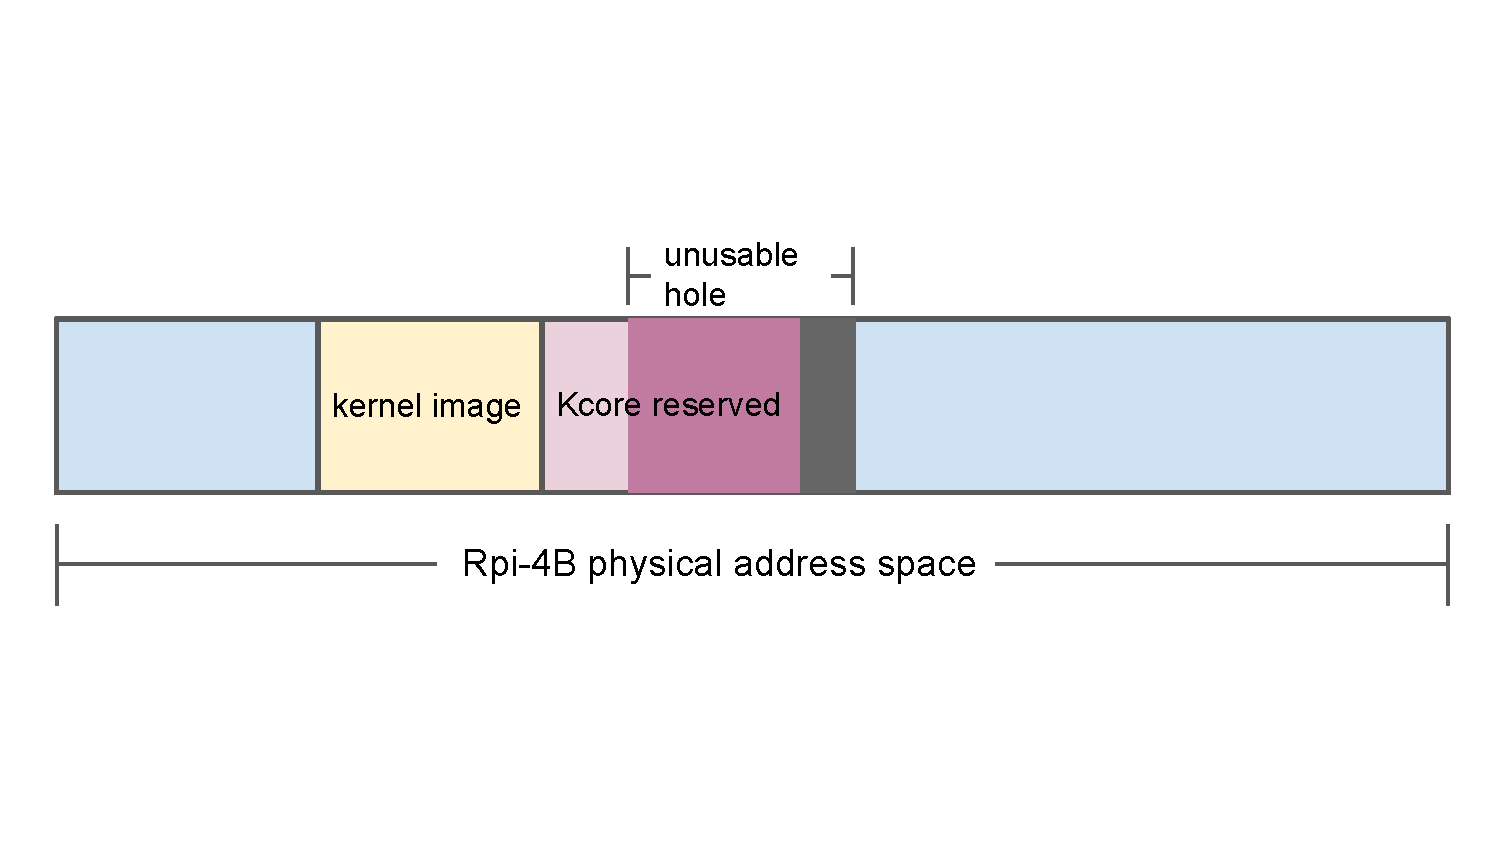
\includegraphics[scale=0.60]{figures/overlap.pdf}
    \caption{Kcore overlaps the unusable hole on Rpi-4B}
    \label{fig:overlap}
\end{figure}

To solve this issue for \rustsec{}, instead of allocating memory in the linker
script, we first locate a range of memory which does not overlap with the
unusable hole of Rpi-4B and the kernel image, then add a new memblock that to
correspond to the \rustcore{}'s private memory. We mark it as reserved by
calling \code{memblock\_reserve}, so that the kernel does not accidentally
access this memory range (\autoref{fig:rcorereserved}).
The global symbols previously defined the Linux kernel linker script have also
been changed to macros that expand into addresses in the reserved range for
\rustsec{}'s \rustcore{} usage.

\begin{figure}[H]
    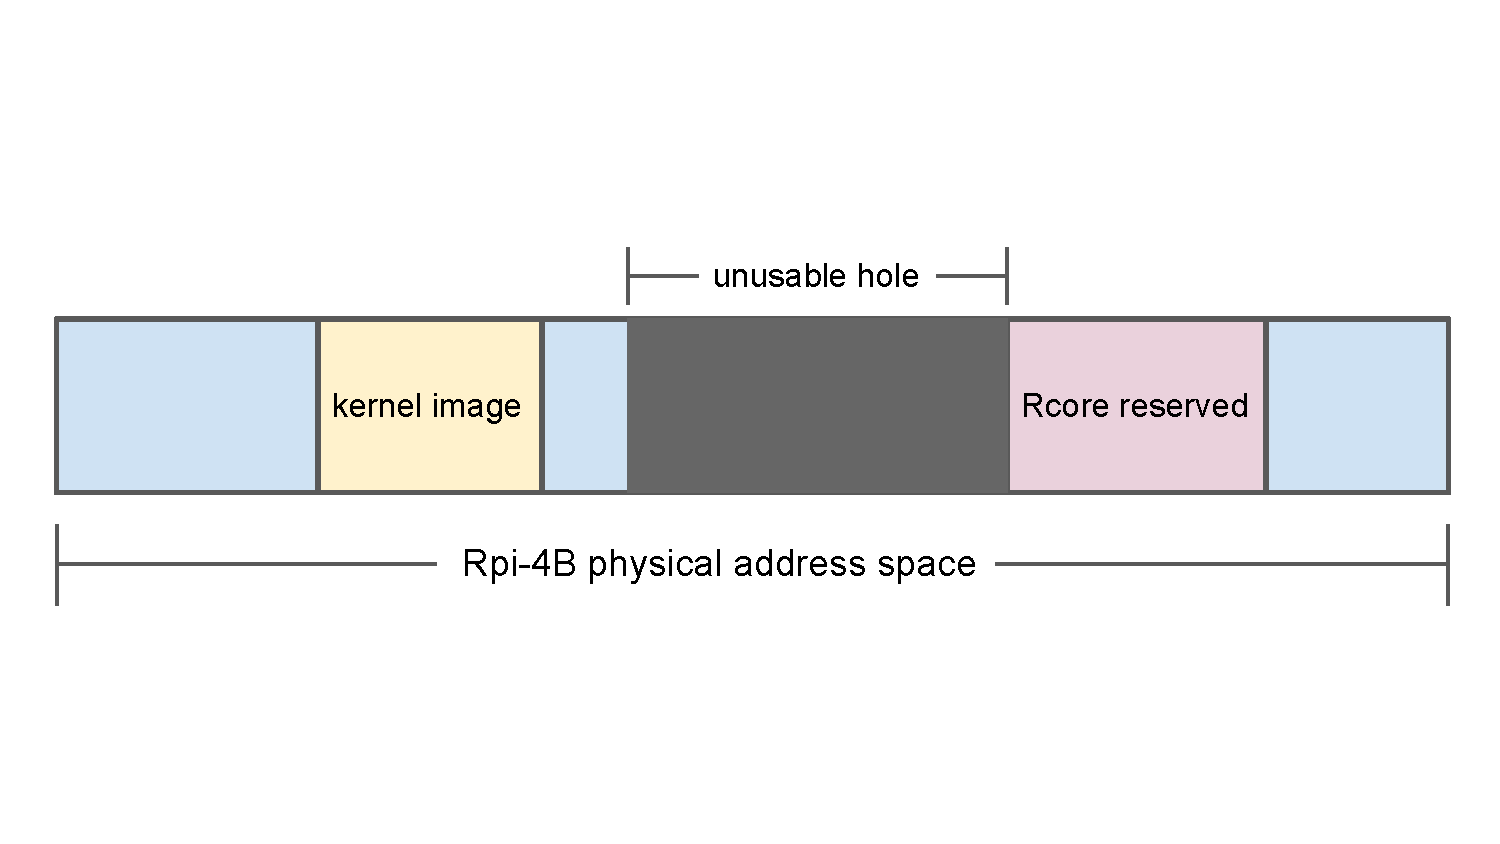
\includegraphics[scale=0.60]{figures/rcore_reserved.pdf}
    \caption{Overlap prevention}
    \label{fig:rcorereserved}
\end{figure}

\section{Rewriting C-based \secore{} into Rust-based \rustcore{}}

%challenge: difficult to do a top-down design due to the difficulty to debug
%and complexity of a hypervisor (is this challenge kinda weak?)
%
%solution: two pass method, first function-by-function rewrite, then remove
%unsafe and redesign after we have a working Rust hypervisor, and leverage
%Rust to achieve a stronger memory region isolation guarantee.

Given the high complexity of the KVM hypervisor and \secore{},
it is clear from the beginning that
a top-down approach to a Rust rewrite would be error-prone and difficult to test.
Therefore, we elected to start the rewriting effort bottom-up,
where all previous C functions in the TCB are rewritten in Rust, one by one.
This incremental approach allows us to test one rewritten function at a time,
reducing the risk of introducing bugs.
%One major downside of this approach is that it is difficult to rewrite a single
%function in a Rust-idiomatic and safe way.
One major downside of this approach is the difficulty of rewriting individual
functions in a manner that adheres to Rust's idiomatic practices.
Furthermore, it may result in a lot of \code{unsafe} blocks.
We solve these issues by adding a second phase to the Rust rewrite;
after the initial function by function rewrite, we removed unnecessary
\code{unsafe} blocks, refactored the code to be more Rust-idiomatic,
and leveraged Rust features to enhance \rustcore{} memory safety.
We discuss the features used to secure \rustcore{} memory accesses in
\autoref{sec:securercore}.


\chapter{Securing \rustcore{} Memory Accesses}
\label{sec:securercore}

%Continues from Code Migration (the redesign after the function-by-function
%rewrite), talk about \rustcore{} here.
%
%Rust has safe and unsafe code -> segregate unsafe code so that most of the
%hypervisor is written in safe Rust

\section{\rustcore{} Memory Regions}
\label{sec:rcoreregions}

\rustcore{}'s memory accesses are categorized into four disjoint regions:
\textit{\rustcore{} Metadata}, \textit{Page Table Pool},
\textit{SMMU Area}, and \textit{Generic Area}.
\rustcore{} metadata and \rustcore{} Page Table pool combined are referred to as
the \textit{\rustcore{} area} in the following.

\textbf{\rustcore{} Area.}
\rustcore{} needs a reserved memory region separated from the host Linux kernel
and all other VMs, named \textit{\rustcore{} area}, to provide its functionality.
The \rustcore{} area comprises the \rustcore{} Metadata and the \rustcore{} Page Table Pool.
The \rustcore{} Page Table Pool, as its name suggests, keeps private pools of physical pages
for NPTs and SMMU page tables so that \rustcore{} has complete control
over the permissions and the virtual-to-physical mappings of the memory
accessed by the host Linux kernel, VMs, and I/O devices. The \rustcore{} metadata,
on the other hand, is used for storing \rustcore{} metadata described in
\autoref{sec:RCO}

\textbf{SMMU Area.}
SMMU is accessed via MMIOs. \rustcore{} unmaps the SMMU
from the host NPT to trap-and-emulate its access to the SMMU. This
approach assures \rustcore{} has exclusive access to the SMMU.

\textbf{Generic Area.}
The \textit{Generic Area} refers to memory outside the \rustcore{} area and the SMMU area.
\rustcore{} needs to access this area to modify memory pages
belonging to the host or guests for VM services, such as zeroing a page
before transferring ownership from a guest back to the host during VM termination.

\begin{figure}[ht]
\centering
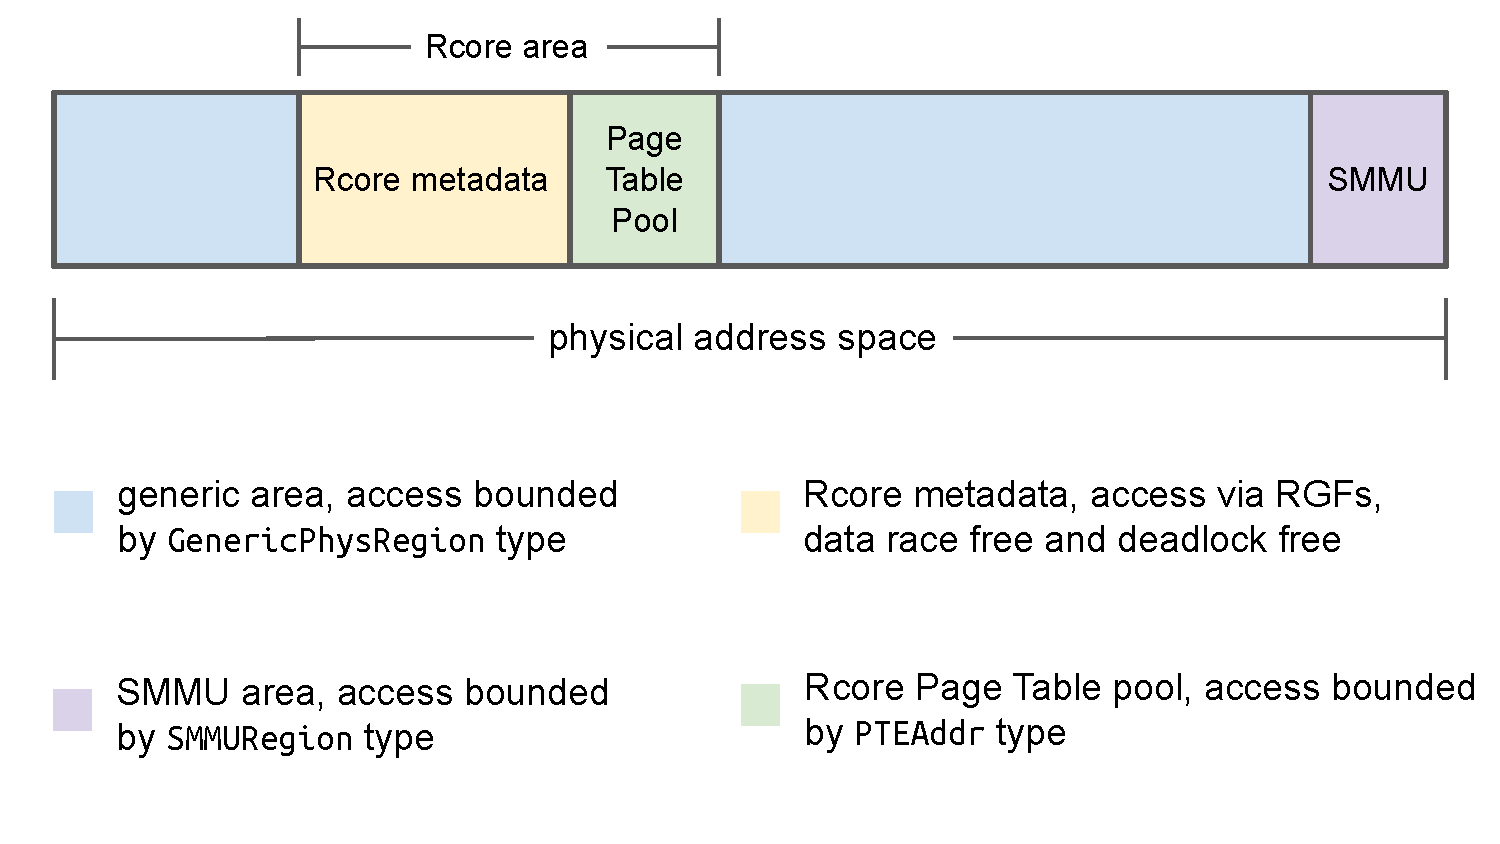
\includegraphics[width=1.00\textwidth]{figures/regions.pdf}
\caption{Memory Regions}
\label{fig:regions}
\end{figure}

\section{\rustcore{} Metadata and Reference Getter Functions}
We aggregate \rustcore{} metadata structures
into a single big structure \code{RcoreMetadata}
(line 1 in \autoref{lst:getternew})
to simplify the memory region used by these metadata.
All CPU cores share metadata in \rustcore{}; some are per CPU.
Fields shared by all CPU cores in \code{RcoreMetadata} are defined as type \code{\lock{}<T>}
(an example is line 3 in \autoref{lst:getternew}),
where \code{T} is the type that actually stores \rustcore{} metadata.
\rustcore{}'s custom \code{\lock{}} is a generic type which can hold any
arbitrary type alongside a lock.
The only way to access the data wrapped in \code{\lock{}} is by calling the
\code{lock} method of \code{\lock{}} reference.
Since there is no existing memory allocator in a hypervisor environment,
we directly inform where in the address space \rustcore{} should use.
Specifically, we pre-defined the address to the instance of \code{RcoreMetadata}
and manually initialize this memory region at boot time,
so it can be used safely thereby.
Using that raw address, we implemented several functions that
transform the raw pointer to \code{RcoreMetadata} into mutable references to
each of its fields and return them to the caller.

We implement a set of reference getter functions (RGFs). \rustcore{}
can use the RGFs to safely access \code{RcoreMetadata} with safe Rust.
%We enable the \funcl{} layer to safely access \code{RcoreMetadata}, without any
%unsafe Rust by implementing a set of reference getter functions (RGFs) that
%the \funcl{} layer can call.
Each RGF returns a mutable reference to one of the fields in \code{RcoreMetadata},
line 10 of \autoref{lst:getternew} is an example of an RGF, it returns the mutable reference
of the type \code{\lock{}<PMemInfo>}. The RGF is implemented by:

\begin{enumerate}
  \item dereference the raw pointer using the \code{*} operator
  \item pick the \code{pmem\_info} field of \code{RcoreMetadata}
  \item take the mutable reference of the field by prepending \code{\&mut}
  \item return the mutable reference
\end{enumerate}

By defining fields of \code{RcoreMetadata} as \code{\lock{}<T>}, and with
the RGFs, most of \rustcore{} is free from directly using raw pointers to access
\rustcore{} metadata, and proper locks are guaranteed to be held when accessing
them.

\begin{listing}[ht]
    \begin{minted}{Rust}
struct RcoreMetadata {
  [...] // other fields omitted
  pub pmem_info: KMutex<PMemInfo>,
  [...] // other fields omitted
}

const RCORE_METADATA_PTR: *mut RcoreMetadata = /* Rcore's memory address */;

// the RGF of pmem_info
pub fn get_pmem_info<T: CanGetPMemInfo>(_: &mut T) -> &mut KMutex<PMemInfo> {
  // SAFETY: The pointer points to an initialized memory.
  // The data is properly wrapped in a KMutex
  // and the caller have the permission to get PMemInfo
  unsafe {
    &mut (*RCORE_METADATA_PTR).pmem_info
  }
}
    \end{minted}
    \caption{\rustcore{} metadata and Reference Getter Function}
    \label{lst:getternew}
    \vspace{-0.2cm}
\end{listing}

\section{Memory Region Isolation}

Raw pointer accesses are prohibited in safe Rust as they easily violate Rust’s
ownership model. As detailed in the upcoming paragraphs, we examine the need
for raw pointers for accessing the four regions described in \autoref{sec:rcoreregions}
and the measures taken to guarantee their isolation,
even when employing unsafe Rust in their implementation.
We also deliberately made the
amount of unsafe code that contains raw pointer accesses small ($\sim$50 LOC).

\textbf{Raw Pointer Access: \rustcore{} Metadata.}
The RGFs return mutable references from a raw pointer, thus encapsulating the
raw pointer usages when the caller wishes to access \rustcore{} metadata
(\code{RcoreMetadata}).
All memory accesses done via RGFs are bounded in the range
from \code{RCORE\-\_\-META\-DATA\-\_\-PTR} to
\code{RCORE\-\_\-META\-DATA\-\_\-PTR + size\-of\-(Rcore\-Metadata)},
as accesses to non-array fields will not go out of bounds,
and Rust automatically adds runtime checks for the indices when array fields are accessed.
We manually check this range is only accessible by \rustcore{} and disjoint
from the page table pool and SMMU area by checking it is within the memory range unmapped from the
host Linux kernel for \rustcore{} and comparing the addresses with the page table pool area and SMMU area.
Hence, it is impossible for \rustcore{} metadata accesses to access
the other three regions accidentally.

\textbf{Raw Pointer Access: Generic Area.}
Generic area accesses are done by calculating raw addresses and writing to them
via raw pointers. Raw pointers are necessary here because system RAM is just a
range of flat address space to \rustcore{}. To ensure that code accessing the
generic area does not accidentally access the \rustcore{} area,
a new type called \code{GenericPhysRegion}
(\autoref{lst:genericphysslice}) has been created, which can only point to a
memory range in the generic area.
\code{GenericPhysRegion} only has one constructor, namely the \code{new}
method at line 2 in~\autoref{lst:genericphysslice}. This method verifies whether
the memory range specified by the arguments (start address \code{start\_addr} and
access size \code{size}) is contained within the bounds of the generic area.
If the specified range overlaps with the \rustcore{} area or the SMMU area, the constructor
returns a \code{None} variant, indicating that the construction has failed.
\autoref{lst:genericusage} shows an example usage of
\code{GenericPhysRegion}, which is a function that takes a physical frame number
(pfn), and clears the contents of the page.
The \code{GenericPhysRegion::new()} function is called at line 2 with the
physical address of the page (\code{pfn << PAGE\_SHIFT}) and its size
(\code{PAGE\_SIZE}) as arguments and returns a type of
\code{Option<GenericPhysRegion>}.
Next, we transform \code{Option} to \code{Result} type through \code{ok\_or}.
and use the \code{?} operator on the \code{Result} type to return the
contained value to \code{page} if it is an \code{Ok} variant.
Otherwise, \code{clear\_page} immediately returns \code{Err\-or}
without executing anything after line 2,
effectively propagating the absence of a value up the call stack.
The caller of \code{Generic\-Phys\-Region::\-new()} gets a
\code{GenericPhysRegion} if the check passes; otherwise,
\code{clear\_page} returns an \code{Error} type.
If successful, the page contents are cleared at line 4.

\begin{listing}[hbtp]
    \begin{minted}{rust}
impl GenericPhysRegion {
  pub fn new(start_addr: usize, size: usize) -> Option<Self> {
    let end = start_addr + size;
    // overlap check
    if (end > RCORE_AREA_START && RCORE_AREA_END > start_addr)
    || (end > SMMU_AREA_START && SMMU_AREA_END > start_addr) {
      return None;
    }
    Some(Self {
      start_addr,
      size,
    })
  }

  // returns a mutable `u8` slice for the caller
  // to access generic area memory
  pub fn as_slice(&self) -> &'static mut [u8] {
    // convert the physical address to the virtual address
    let va = pa_to_va(self.start_addr);
    unsafe {
      core::slice::from_raw_parts_mut(
        va as *mut u8, self.size,
      )
    }
  }
}
    \end{minted}
    \caption{\texttt{GenericPhysRegion} guarantees that every instance points to a valid generic area range}
    \label{lst:genericphysslice}
    \vspace{-0.2cm}
\end{listing}

\begin{listing}[hbtp]
    \begin{minted}{rust}
fn clear_page(pfn: usize) -> Result<()> {
  let page = GenericPhysRegion::new(pfn << PAGE_SHIFT, PAGE_SIZE).ok_or(Error::InvalidPfn)?;
  // the `fill` method for type &[u8] fills the slice with the value passed in
  page.as_slice().fill(0);
  Ok(())
}
    \end{minted}
    \caption{Example usage of \texttt{GenericPhysRegion}}
    \label{lst:genericusage}
    \vspace{-0.2cm}
\end{listing}

\textbf{Raw Pointer Access: Page Table Pool.}
\rustcore{} manages the host's and each VM's NPTs to control their access to
physical memory. SMMU page tables control I/O devices' memory access.
We also leveraged Rust's type system and created the
type \code{PTEAddr} (Page Table Entry Address). Each instance of type \code{PTEAddr}
points to an entry in the \rustcore{} Page Table Pool region.
Similar to \code{GenericPhysRegion}, \code{PTEAddr}'s constructor verifies whether the physical address provided as an
argument for the constructor is within the page table pool region in the \rustcore{}
area. If the address falls within the range, it is translated to the
corresponding virtual address and stored in a field of the
\code{PTEAddr} instance. Otherwise, the construction fails, and a
\code{None} is returned.
This type encapsulates the raw pointer address translation and bound
checks so for example the NPT walking code,
can guarantee it is accessing NPT entries in the
\rustcore{} page table pool area by using \code{PTEAddr}.

\textbf{Raw Pointer Access: SMMU.}
In a manner analogous to the generic area and page table pool, the type
\code{SMMURegion} for accessing SMMU is created.
\rustcore{} uses \code{SMMURegion} whenever it reads or writes SMMU registers.
\code{SMMURegion}'s \code{new} method takes the MMIO address and
verifies its inclusion within the SMMU region.
By consistently utilizing this type for SMMU accesses, SMMU accesses are
guaranteed to access the correct address region.

\chapter{Evaluation}
\label{sec:eval}

We evaluated the performance of various application benchmarks
on a VM running on \rustsec{}, SeKVM, and mainline KVM.
We also tested the same
benchmarks on bare metal environment performances to establish a baseline
reference of the benchmark results. The workloads were run on the Raspberry
Pi 4 model B development board, with a Broadcom BCM2711, quad-core
Cortex-A72 (ARM v8) 64-bit SoC at 1.5GHz, 4GB of RAM, and a 1 GbE NIC device.

\rustsec{}, SeKVM, and the mainline KVM are all based on Linux 5.15.
QEMU v4.0.0 was used to start the virtual machines on Ubuntu 20.04. The guest
kernels also used Linux 5.15, and all kernels tested employed the same 
configuration. We requested the authors of~\cite{hypsec} and got a patch for
the Linux guest kernel to enable virtio.
\code{rustc} version 1.68.0-nightly was used to compile \rustcore{},
while clang 15.0.0 was used to compile the remaining components of
\rustsec{}, SeKVM, and the mainline KVM.
2 physical CPUs and 1 GB of RAM is configured for the bare
metal setup, and each VM is equipped with 2 virtual CPUs , and 1 GB of RAM.

We ran the benchmarks listed in \autoref{tab:benchmark} in VMs on
\rustsec{}, SeKVM, and the mainline KVM. \autoref{fig:eval} shows the normalized
results. In \autoref{fig:eval} we normalized the results to bare-metal
performance. 1.00 refers to no virtualization overhead, and
a higher value means higher overhead. The performance on real application
workloads show modest overhead overall for \rustsec{} compared to SeKVM and
mainline KVM. The overhead for \rustsec{} in most of the cases is less than
10\% compared to mainline KVM.
In the \code{TCP\_MAERTS} benchmark, all four experimental setups saturated the
1GbE NIC on the Raspberry Pi 4 model B. Additionally, experimental error had a
more noticeable impact during the measurement of the bare-metal setup, making
its performance the worst.
For \rustsec{}, \code{TCP\_RR} and the YCSB-Redis benchmarks experienced higher
overhead compared to mainline KVM at around 8\% and 14\%, respectively.
\code{TCP\_RR} and YCSB-Redis are benchmarks that both send a lot of small
packets, causing many VM exits. Hence, the bare-metal performance
is roughly twice as good as the VMs, amplifying the difference between mainline
KVM and \rustsec{} when plotting \autoref{fig:eval}.
%In fact, if the overhead are plotted by normalizing against the
%performance of mainline KVM (\autoref{fig:eval2}), all benchmarks run on
%\rustsec{} experience an overhead less than 10\% compared to mainline KVM.
In fact, when the overhead is normalized against the performance of the
mainline KVM (\autoref{fig:eval2}), all benchmarks executed on \rustsec{}
demonstrate an overhead of less than 10\% in comparison.
\rustsec{} performs nearly as well as mainline KVM in
CPU bound benchmarks and bulk data network performance benchmarks
(\code{TCP\_MAERTS}, \code{TCP\_STREAM}) since
the workloads require minimal to no VM exits.
The discrepancy arises in \code{TCP\_RR}, Apache, Memcached,
and YCSB-Redis, which involve a higher number of VM exits due to their frequent
small network transmissions. Both SeKVM and \rustsec{} execute additional logic
in EL2 to ensure VM data confidentiality and integrity, resulting in increased
overhead in VM exits compared to mainline KVM.
%The worst overhead for \rustsec{} compared to mainline KVM occurs for the
%YCSB-Redis benchmark at around 14\%.
%Various system noise factors e.g. caches, kernel thread wakeups, and dynamic
%voltage frequency scaling might also come into play.

\begin{table}
\centering
\footnotesize
\begin{tabular}{ |p{0.2\linewidth}|p{0.7\linewidth}| }
 \hline
 \small{\textbf{Name}} & \small{\textbf{Description}} \\
 \hline
 \small{Kernbench} & \small{Compilation of the Linux 6.0 kernel using \code{tinyconfig} for Arm with GCC 9.4.0.} \\
 \hline
 \small{Hackbench} & \small{\code{hackbench}~\cite{hackbench} using Unix domain sockets and 50 process groups running in 50 loops.} \\
 \hline
 \small{Netperf} & \small{\code{netperf}~\cite{netperf} v2.6.0 running the netserver on the server and the client with its default parameters in three modes: TCP\_STREAM (throughput), TCP\_MAERTS (throughput), and TCP\_RR (latency).} \\
 \hline
 \small{Apache} & \small{\code{Apache} v2.4.41 Web server running \code{ApacheBench}~\cite{ab} v2.3 on the remote client, which measures the number of handled requests per second when serving the 41 KB index.html file of the GCC 4.4 manual using 100 concurrent requests.} \\
 \hline
 \small{Memcached} & \small{\code{memcached} v1.5.22 using the \code{memtier}~\cite{memtier} benchmark v1.2.3 with its default parameters.} \\
 \hline
 \small{YCSB-Redis} & \small{\code{redis} v7.0.11 using the \code{YCSB}~\cite{YCSB, YCSB2} benchmark v0.17.0 with its default parameters.} \\
 \hline
\end{tabular}
\vspace{0.3cm}
\caption{Application Benchmarks}
\label{tab:benchmark}
\end{table}

\begin{figure}[hbtp]
    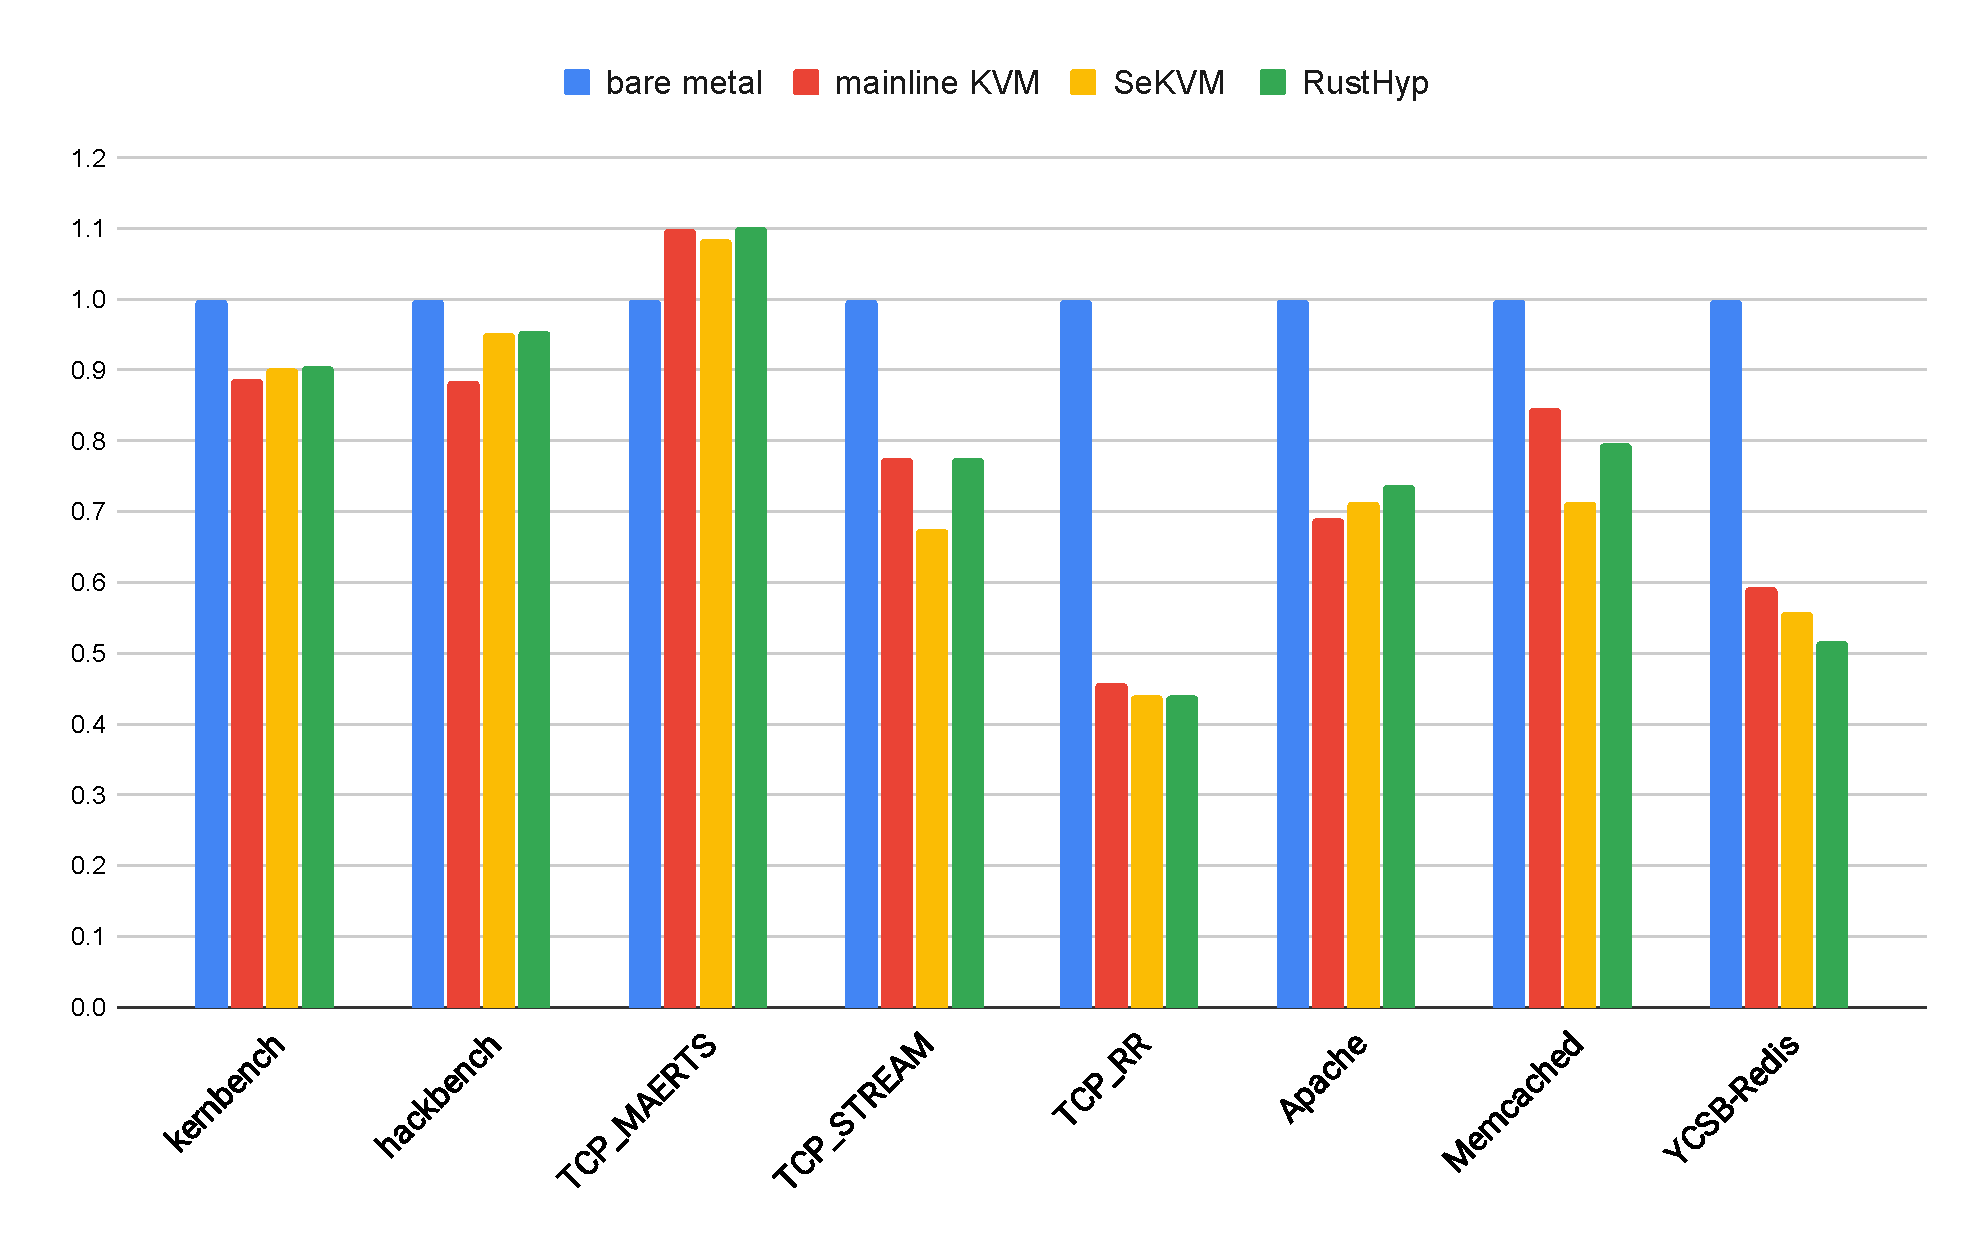
\includegraphics[scale=0.45]{figures/eval.pdf}
    \caption{Application Benchmark Performance: Overhead normalized to the bare-metal setup}
    \label{fig:eval}
\end{figure}

\begin{figure}[hbtp]
    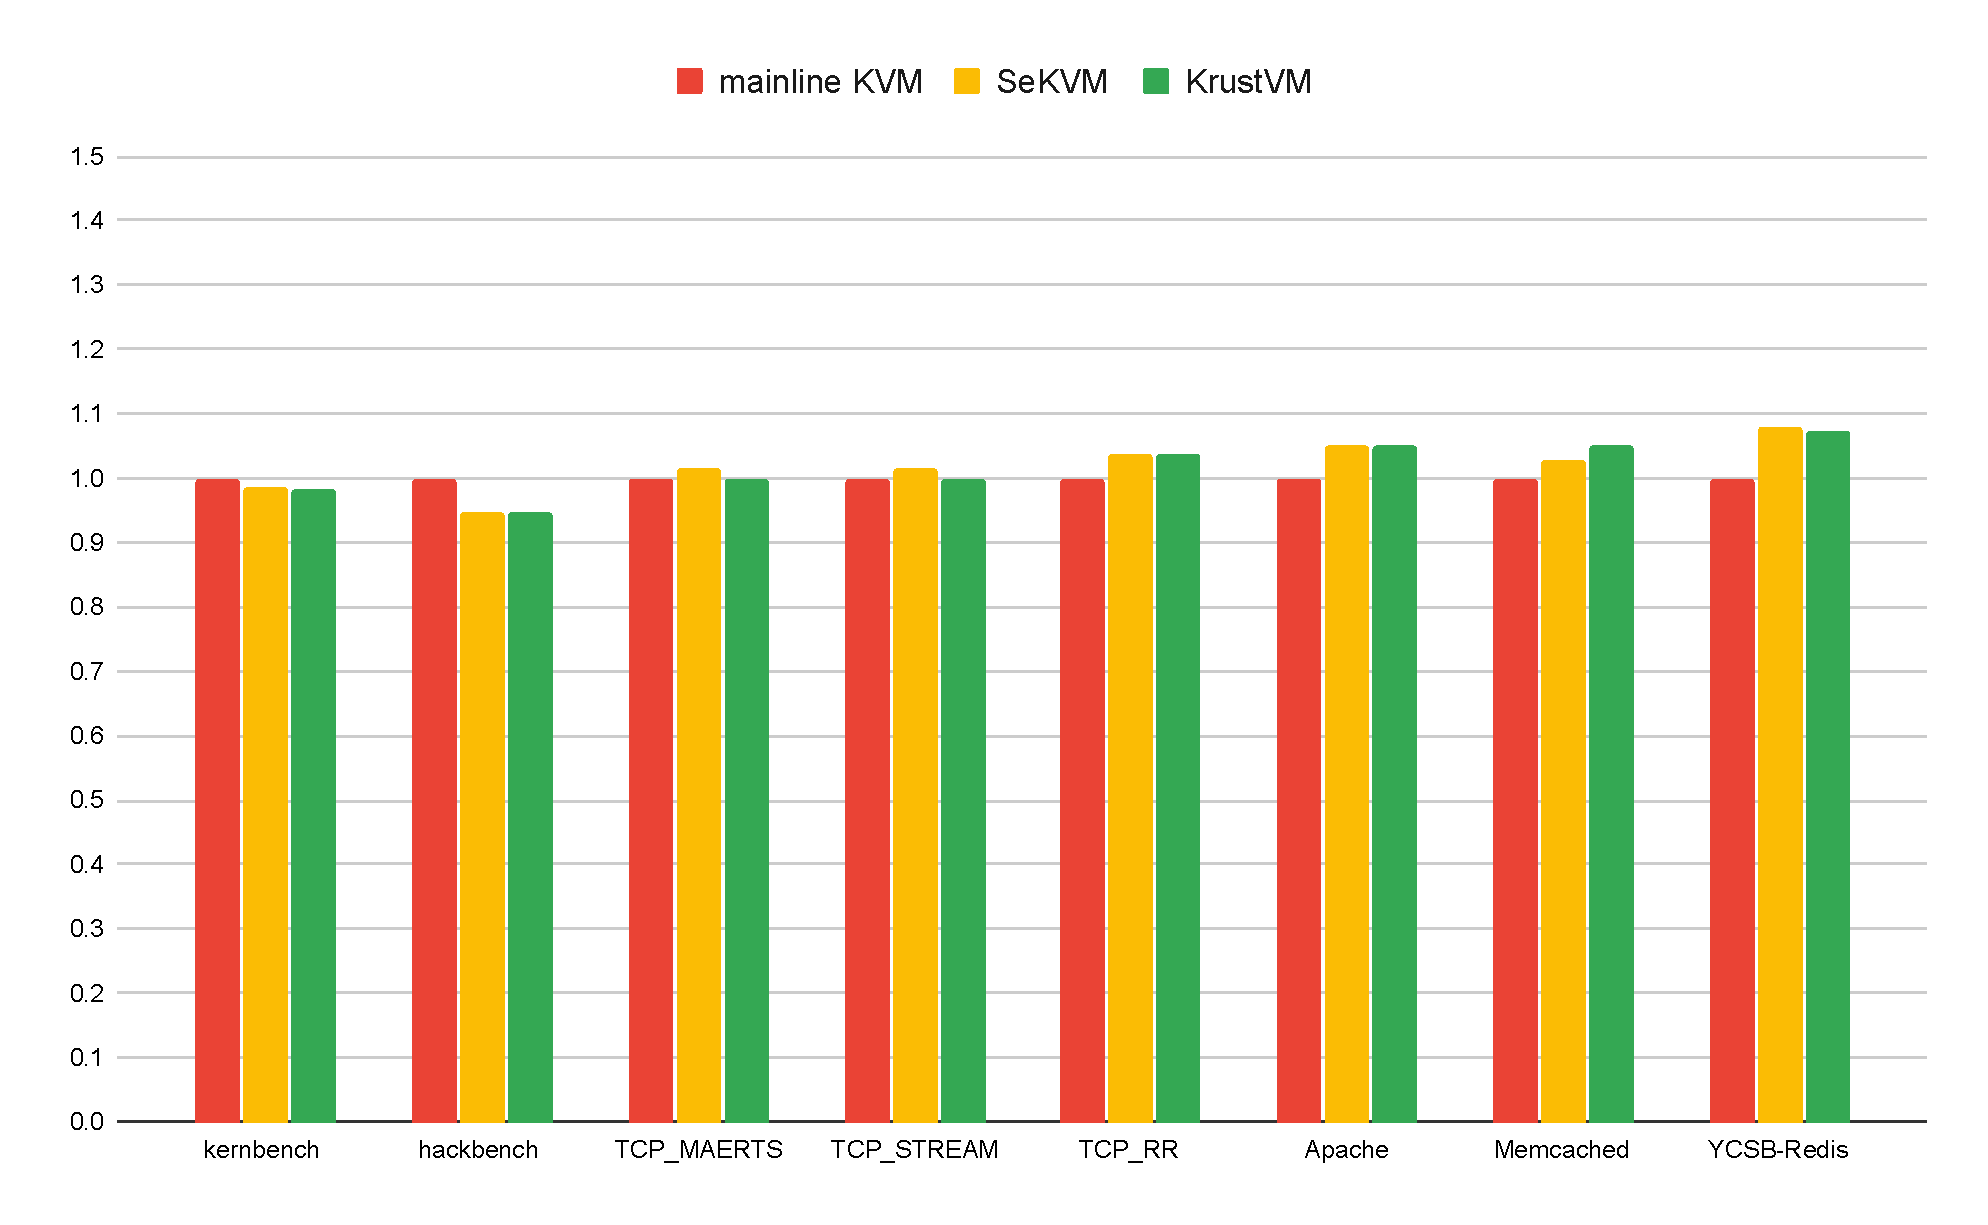
\includegraphics[scale=0.45]{figures/eval2.pdf}
    \caption{Application Benchmark Performance: Overhead normalized to mainline KVM}
    \label{fig:eval2}
\end{figure}

% !TeX root = ../main.tex

\chapter{Conclusions}



% 參考文獻
% References
\refmatter
\bibliographystyle{abbrv}
\bibliography{back/references}

% 附錄
% Appendices
\input{back/appendix01}

\end{document}
